% !Mode:: "TeX:UTF-8"
\chapter{The New Quantum Universe}
[英]安东尼.黑\ 帕特里克.沃尔特斯著, 雷奕安译

这本书的姐妹篇<<爱因斯坦的镜子>>

物理学家, 就像一个好侦探一样, 仔细分析各种证据, 遵循福尔摩斯说过的一句格言:"当你把不可能的事情都排出了以后, 剩下的选择,不管看起来多么不太可能, 一顶是对的."  \\
光子的本质是量子力学的

\textbf{电子的双缝实验}\\
\fbox{Result: 在没有观察光源时, 电子双缝实验发生干涉, 而有观察光源时, 干涉图案消失.}\\
打开和不打开用来观察电子的光源将导致不同的结果! 这一明显的疑惑来自于光子本身的量子属性. 光, 跟电子一样, 是以确定的叫光子的能量块的方式过来的. 为了看见一个物体, 必须至少有一个光子从这个物体上反弹回来. 这正是问题的症结. 但我们将光照射到子弹上时, 子弹的运动不会发生可以察觉的改变. 因为一个单个的光子的能量和子弹的能量相比太小了. 而电子确实非常细小的量子对象. 光照在点子上会给电子一个猛击, 从而显著改变电子自身的运动状态. 更仔细的分析发现,这一扰动总是正好足够破坏整个干涉图案.
\bigskip

\section{海森堡不确定原理}
$$
\Delta x\times \Delta p \geq \hbar
$$
实验测量的精度存在原则上的极限. 在量子世界里, 扰动(比如光子造成的扰动)是无法忽略的, 这就是海森堡不确定原理的本质.\\
为了精确测量粒子的位置, 就必须使用波长很短的光,因为光的波长决定了无门能将粒子定位在某一定范围的最小长度. 而很短的波长的光有很高的频率, 光子的能力$E=h\nu$, 高频率的
光子达到系统上, 会给量子体系一个很大的推动. 出于同样的原因, 如果想精确测得动量, 我们只能给体系一个很小的推动, 根据普朗克的公式, 这就意味着只能使用低频率的光. 而低频率的光意味着很长的波长, 这样反过来就意味着位置测量的很大不确定性.
\bigskip

\textbf{不确定性与照相术}\\
眼睛就是一个很好的光子探测器: 一个光子就可以激发一个视网膜细胞. 当然, 一般情况下, 很多光子还没有到达视网膜, 就被眼睛吸收了\textit{组成眼睛的很多其他细胞的原子也吸收光子}.
出于这一原因, 大约只有百分之几进入到眼睛的光子真正被眼睛探测到. 显然, 看东西这种化学反应必须是可逆的\textit{否则, 看到一种东西之后, 不回复到之前的状态就看不到新的东西了}---实际上, 大约0.1 秒以后视觉细胞就会回到之前的正常状态. \\
照相术通过把这种化学变化永久保存在感光乳剂里, 克服了眼睛的这种限制.\\
感光胶片里面有很多银化物颗粒, 颗粒里面的银是离子化的. 当光子被乳液吸收的时候, 有时会放出一个电子, 就像光电效应一样. 这个电子会被一个阴离子吸引, 结合成一个电中性的银原子.
游离出来的银原子被含有银离子的化合物包围, 这是不稳定的. 银原子很容易放出电子, 重新变成银离子. 如果在他变成银离子之前, 又有一些光子在他的附近产生了好几个银原子, 这时就会形成一个由几个银原子组成的稳定"显影中心", 而照片就是由很多微小的显影中心形成的.\\
拍照时, 曝光时间极短时, 只有几个光子进入, 那么照片上出现的是一些随机点, 但当曝光时间增加, 进入的光子数也增加, 我们看到显影中心更多的出现在以后图像上很亮的地方. 因此,即使在拍照这样一件非常普通的行动中, 我们也能看到光的量子的, 随机的自然属性.
\bigskip

\textbf{分形: 奇妙的数学}\\
在所有的尺度下看起来都很相似(自相似)\\
当我们观察量子在一段时间内的运动路径时, 发现当我们不断增加放大倍数, 这些量子路径看起来都是锯齿状的,而且都是非常相似的.\\
海岸线是一条分形曲线, 长度取决于我们在什么尺度下测量. 这种现象也是一些百科全书在给出一些国家之间的陆地边界线长度时, 数据不同的部分原因.\\
\textbf{分数维}:描述一条曲线的不规则程度. 一条平滑的曲线的分数维$D=1$, 跟普通的维数一样, 而一条曲线确实不规则, 越是到处有着尖角, 他的分数维就越接近$D=2$, $D=2$ 就是一条非常不规则的曲线, 差不多把一个两维空间都填满了.\\
利用分型理论可以用计算机生成人造风景, 已经是现代电影制造业的一种标准技巧了.

\section{薛定谔和物质波}
$$
E\phi = -\dfrac{\hbar^2}{2m} \frac{d^2 \phi}{dx^2} + V\phi
$$
$$
\lambda = h/p
$$

\section{原子核模型}
电子的数目, 或者等价的说, 质子的数目, 决定了不同元素的化学性质.\par
在通常的温度下, 气体里原子的碰撞一般不足以激发很多的原子, 因为基态与第一激发态之间的能量差很大. 因此在室温下, 大多数原子都处于基态. 基态与任意一个激发态之间的能量差都很大, 相应的光子的频率处于紫外波段, 而不是可见光波段, 因此, 可见光直接穿透很多气体, 而不被吸收. 这就是为什么大多数气体对可见光来说是透明的原因.\par
\textbf{彭宁离子阱}:他能把电子限制在真空中两块带有负电的金属盘中间. 金属盘周围有磁场, 用来防止电子从阱的旁边溢出. 利用一个带负电的金属叉子可以把电子放置到阱中.
通过检测例子在阱中的来回震荡阱, 可以确认粒子的存在. 实际做法是让电子一个一个不断逃出阱外, 知道最后只剩下一个电子.

\section{量子隧道效应}
对时间和能量的测量也存在一个类似的关系
$$
\Delta E \Delta t \geq \hbar
$$
虽然经典意义上, 我们不可能在不违反能量守恒的前提下改变总能量, 但是在量子力学里, 如果时间不确定性是$\Delta t$, 我们无法把能量测量的比$\Delta E = \hbar /\Delta t$精确.
粗略的说, 我们能借到一些能量$\Delta E$来越过壁垒, 只要我们在时间$\Delta t = \hbar / \Delta E$内把能量还回去. 如果势垒太高或者太宽, 隧穿的可能性就会变得非常小.

扫描隧道显微镜

\subsection{核反应}
加莫夫最早提出用量子隧道效应解释阿尔法衰变. 因为阿尔法粒子非常稳定, 我们可以认为它本来就在原子核里存在, 处在一个由别的核子形成的势场之中. 
艾尔法粒子可以以隧道效应的方式从原子核里跑出来, 引起原子核衰变.

\begin{figure}[htbp]
		\centering
		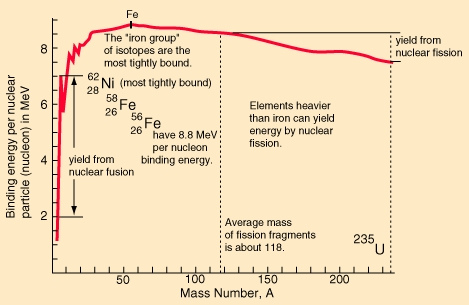
\includegraphics[scale = 0.5]{association_energy}
		\caption{每个核子的平均结合能}
		\label{fig.nuclear.association}
\end{figure}
从
\ref{fig.nuclear.association},
我们可以看出, 结合能从2兆电子伏特(氘的结合能)开始, 不断上升, 到铁的时候达到最大值, 即每个核子$8.8$兆电子伏特, 
然后逐渐下降到重核(铀及以上元素)的每个核子$7.5$兆电子伏特.
注意, 阿尔法粒子(氦原子核)与附近的元素相比, 特别稳定. 这就是为什么在重核中, 会形成阿尔法粒子, 并通过隧道效应跑出来, 因而引发原子核放射性衰变.

结合能最大的铁所处的位置说明了, 有两种方式可以把原子核里的能量释放出来.一种是聚变(两个比较轻的原子核结合在一起形成一个重核), 另一种是衰变(一个很重的核裂解成两个较轻的的核).
这两种过程释放出来的结合能, 将以最终生成粒子的动能的形式表现出来.

一个典型的核聚变的反应的例子:
$$^2H + ^3H \rightarrow ^4H_e + n$$
$$\eqnote{氘} + \eqnote{氚} \rightarrow \eqnote{氦} + \eqnote{中子}$$
这一反应的潜在释放能量是17.6兆电子伏特. 但如果用这种方式来发电的话, 会有一个问题, 那就是很难建立一个环境, 让这个反应持续进行, 原因来自于我们熟悉的昆仑排斥力.
库伦排斥力会将相互接近的原子核推开, 如果用加速器把氘核加速到比库仑排斥势高的能量, 很容易引发这一核反应, 但是如果用这种方式来大规模产生能量, 经济上是不可行的.\\
人们提出了另外一个种想法, 把反应原料加热到非常的温度, 以至于这种高热气体或者叫做等离子体里发生的普遍碰撞中, 反应物有足够的动能发生核反应. 但是如何产生所需的高温, 还没有好的办法.

\section{泡利与元素}
如果我们让另一个氢原子靠近第一个氢原子, 会发生什么呢? \\
如果两个电子的自旋都向上, 泡利不相容原理将禁止两个氢原子靠近, 因为两个电子的波函数会重叠, 波函数重叠就意味着两个电子会处于同一个量子态. 
如果两个电子的自选方向相反, 他们就可以互相靠近, 并且实际情况是, 两个电子大部分时间都呆在两个氢原子核之间. 
这样就在两个氢原子之间产生了一个束缚力, 形成一个稳定的氢分子. 这种化学键, 也就是两个电子被分子中两个原子共享形成的化学键, 叫做共价键. 
正是泡利不相容原理, 说明了为什么氢原子是化学活泼的, 为什么两个氢原子能够形成一个氢分子$H_2$. 
注意, 同样是泡利不相容原理, 禁止了第三个氢原子与氢分子$H_2$ 再形成共价键, 因为两个能量最低的自旋态已经都被占据了.

下一个最简单的原子是氦, 有两个电子, 都填布在最低的1S能级上, 他们的自旋必须相反. 
因为1S 能级上已经没有地方容纳更多的电子了, 泡利不相容原理将禁止别的电子靠近氦原子, 就像他对氢分子那样, 
因此我们可以预料到氦原子的化学性质很不活泼, 实际上他就是一种惰性气体.

\subsection{金属, 绝缘体与半导体}
从某种角度来说, 金属可以看成是共价键的一个极端形式, 其中的传到电子被整块金属中所有的原子共享.

\begin{figure}[htbp]
		\centering
		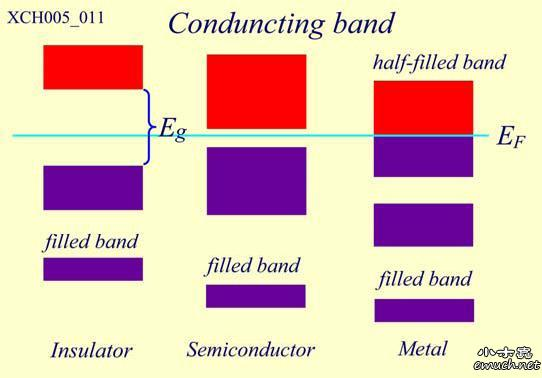
\includegraphics[scale = 0.5]{conduction_band}
		\caption{金属, 绝缘体与半导体的能带}
		\label{fig.paoli.conduction}
\end{figure}
电子热激发对于绝缘体和半导体的导电性质就很关键了.
假设我们有一中材料, 它的基态是一个完全占据的能带加上一个在它上方的完全空闲的能带. 
如果这两个能带之间的间隙(能隙)很大, 如图\ref{fig.paoli.conduction}所示, 几乎没有电子能够通过碰撞而获得足够的能量跳到上面的能带上.
因此, 当给这种材料加上一个电压时, 电子所处的能级附近没有空闲的能级让电子获取少量的能量跳过去 --- 因为泡利不允许两个电子占据同一个量子态. 
低的能级已经满了, 高的能带又离得太远, 电子跳不上去. 这就是绝缘体的情形, 在上面的传到能带中, 本质上不存在自由传到电子,因此就无法出现传到电流.

半导体: 它是一种能带结构和绝缘体类似的材料, 但是上下两个能带之间的能隙比绝缘体要小得多. 在常温下, 有显著数目的电子被激发到上面的导带中. 
当加上一个电压之后, 上面的导带已经有比较多的电子, 电子获取外加电场提供的能量, 也有足够的空能级可以利用.下面的能带中也有一些空能级, 也可以参与导电过程. 
这样, 半导体能够相当容易的传到电流, 而且他们的导电性能跟温度有很大的关系.

\subsection{晶体管与微电子}
我们可以根据需要调节半导体的导电性能, 调节的办法是在半导体中掺入大约百万分之一的适当杂质原子.

锗和硅都有4个价电子, 绝大多数都填入了价带中的$4N$个态中, 把价带几乎占满, 价带上面是几乎全空的导带. 
如果我们引入一个杂质, 比如磷, 磷有$5$个价电子, 那么, 因为只需要4 个电子形成晶格的4 个共价键, 多出来的一个电子很容易离开磷原子, 成为一个导电电子. 
类似的, 如果我们引入的杂质只有3 个价电子, 比如硼, 在晶格中就会却是一个共价键, 这时硼就很容易从价带中俘获一个电子, 在价带中留下一个空穴, 空穴也可以被用来导电.

磷原子在紧靠导带下面形成一个施主态(贡献一个电子的态), 这些电子只需要一个很小的能量就可以跳到导带上. 以这种形式掺杂的半导体叫做$n$型半导体.\par
硼原子在紧靠导带下面形成一个受主态(接受一个电子的态), 在室温下, 电子很容易被激发到这些态上. 以这种形式掺杂的半导体叫做$p$型半导体.

\section{量子合作和超流体}
如果两列波之间有一个固定的相位差, 我们就说这两列波相干.\\
两个不同原子光源发出的光, 不会表现出干涉效应, 我们说他们不相干. 每个光源发出的光都是由很多不同原子发出的, 每个原子发出光子的时刻不一样. 
也就是, 每个光源发出的光, 都是由很多个相位不同的光波组成的. 因此, 两个这种光源发出来的光没有固定的相位差, 所有微弱的干涉效应都被掩盖了.

与此相反, 激光有一个显著的特点, 就是从许多不同的原子辐射出来的光的相位是相同的. 正是激光的这种相干性, 才使得激光束可以将光能高度集中, 聚焦在一个很小的点上.\\
laser,light amplification by stimulated emission of radiation

受激辐射: 如果一个能量合适的光子, 照射到一个激发的原子上, 原子会被动的跃迁到低能态上.\\
处于激发态的原子当然自己也会或早或迟的跃迁到低能态上, 可是受到一个辐射的激励时, 这个过程提前发生了.\\
这种辐射出的光子, 与引起辐射光子的相位完全相同, 
这是因为, 原来光波的变化电磁场, 引起受激原子的电荷分布同步震荡, 发射出来的光子相位完全相同, 也就是说他们是相干的, 并且他们的传播方向与激发光子完全相同.

理论非常完美, 但是要利用这一机制产生出足够强度的激光, 让大多数原子处于激发态而不是基态(叫做\textbf{布局逆转}), 这不是一项简单的事情.

激光一个有趣的应用是\textbf{三维摄影(又叫全息摄影)}\\
一束激光通过一个半透镜分成两束, 其中一束射向被拍摄物体, 散射光被照相底片记录; 另一束光不经过与物体的散射, 而直接射向照相底片. 由于激光是相干光, 这两束光会互相干涉.
照相底片记录的是这两束光相遇时的干涉图案. 全息摄影不像普通摄影那样, 只记录光照到照相底片上的强度, 全息摄影还记录了散射光的相位信息, 因为它记录的是干涉图. 
因此全息图包含了从被拍摄物体上过来的所有光学信息. 一张全息图片一点都不像被拍摄的物体, 他看起来是一张脏兮兮的, 由很多随机点构成的图. 
可是, 当用激光来照射这张全息图的时候, 我们就可以看到被拍摄物体的一张完美的三维复制画面. 
而且, 如果你改变观察位置, 从不同角度看这张图, 你能看见图像里各种东西的相对位置, 就像看见了原始被拍摄物体一样. 
特别地, 全息图上从某个角度看被挡住了的物体, 换个角度就可以看到了.

\subsection{费米子与玻色子}
Toutes les particules \'el\'ementaires d\'ecouvertes \`a ce jour sont soit des bosons, soit des fermions.\par

un grand nombre de particules : les fermions sont des particules qui ob\'eissent \`a la statistique de Fermi-Dirac alors que les bosons ob\'eissent \`a la statistique de Bose-Einstein.\\
la loi statistique Fermi-Dirac : quand on \'echange deux fermions, la fonction d'onde change de signe.
物质粒子都是由费米子构成,而玻色子则是媒介子

玻色子包括:
\begin{itemize}
\item 胶子 - 强相互作用的媒介粒子,自旋为1,有8种
\item 光子 - 电磁相互作用的媒介粒子,自旋为1,只有1种
\item W 及 Z 玻色子 - 弱相互作用的媒介粒子,自旋为1,有3种
\item 引力子 - 引力相互作用的媒介粒子,自旋为2,只有1种,尚未被发现
\item 希格斯玻色子 - 自旋为0,目前只发现1种
\item 介子 - 由两个费米子-夸克组成的强子.
\item 由偶数个核子组成的原子核.因为质子和中子都是费米子,故含偶数个核子的原子核是自旋为整数的玻色子.
\item 声子 - 请参阅固体物理学
\end{itemize}

\textbf{宏观的玻色子现象}\\
实验证实: 费米子数目为偶数的元素, 表现为玻色子; 费米子数目为奇数的元素,服从泡利不相容原理, 表现出像费米子.

la condensation de Bose-Einstein玻色-爱因斯坦凝聚: 是玻色子原子在冷却到绝对零度附近时所呈现出的一种气态的、超流性的物态,几乎全部原子都聚集到能量最低的量子态,
形成一个宏观的量子状态  occupent un unique \'etat quantique de plus basse \'energie (\'etat fondamental)

la population macroscopique d'un mode unique de photon dans un laser
大量的光子(玻色子)处于同一个量子状态

虹膜输运现象 P123

\textbf{冷原子}\\
超流体的液氦需要氦原子间有量子协作. 这种类型的波色-爱因斯坦凝聚发生在原子已经处于液态时, 如果是气体, 在凝聚为液滴, 或者冻结为固体之前, 
可不可以发生波色-爱因斯坦凝聚呢? 要产生这种凝聚, 原子之间的距离必须足够大, 以免凝结成液体, 但是距离又不能太大, 以至于无法产生波色-爱因斯坦凝聚.

\section{量子跃迁}
在物理学中使用复数, 是一种功能强大的工具, 可是, 实验中测量到的量都是让我们放心的"实"数, 与此相反, 薛定谔的波函数可以是复数的, 显然不可能是一个可以直接观测的量.

几率概念进入了物理学, 成为了量子理论的本质的, 内在的局限. 当然, 经典物理中也有几率概念, 但是仅仅是一种"现实上"的限制, 而不是要了解一个体系的本质的, "原则上"的限制.
例如抛硬币这个例子, 我们通常假定硬币落地时, 正面和反面朝上的几率是相同的. "现实上", 我们无法预言哪种结果会发生, 
但是,"原则上", 根据经典物理定理, 如果我们对硬币的初始精确状态了解的足够详细, 并且将所有作用在硬币上的各种力精确的计算进去, 我们能够计算出最后的结果. 
与此相反, 根据量子力学, 我们永远也不能逃脱几率的限制.

\subsection{光子与偏振光}
帕斯库尔`乔丹是量子力学发展早期的一些论文的作者, 他说:"测量不仅破坏了被测量的东西, 还生成了被测量的东西".

实验: 一个静止的原子被激发后同时放出两个光子, 这两个光子沿相反方向射出, 他们的偏振状态可以通过一对偏振片测出. 我们得到了如下结果:
\begin{itemize}
	\item 如果两个偏振片都垂直放置在V方向, 两个光子总是通过偏振片射出
	\item 如果两个偏振片都垂直放置在H方向, 两个光子总是通过偏振片射出
	\item 如果两个偏振片分别放置在V方向和H方向, 我们永远也看不到两个光子同时通过
\end{itemize}
换句话说, 我们能看见VV光子对和HH光子对, 但是看不到VH或者HV光子对.\\
爱因斯坦希望的解释: 光子的偏振状态实际上早就已经确定下来了, 就是同方向的.\\
另外一个解释, 似乎需要光子之间有某种神秘的"超距"作用, 也就是, 一旦一个光子的偏振状态被测量出来为V或H, 另一个光子立即将自己的偏振状态改成与它一致.\\
物理学家们不喜欢超距作用, 他们更愿意相信因果关系.

\subsection{瞬时的信息坍缩}
波函数坍缩,是微观领域的现象.微观领域的物质具有波粒二象性,表现在空间分布和动量都是以一定概率存在的,比如"电子云",我们称之为波函数.当我们用物理方式对其进行测量时(同时必然对其干扰),物质随机选择一个单一结果表现出来.如果我们把波函数比作是骰子的话(比如电子云),那么"波函数坍缩"就是骰子落地(比如打在屏幕上显示为一个点的电子).\par
波函数从叠加态坍缩成A或A非至少从某种意义上符合最大熵(最大信息量)原理.\par
当我们要测量粒子的动量的时候,粒子不一定刚好处于动量的本征态,这个态可以表示为动量本征态的叠加(动量本征态组成一组完备的希尔伯特空间的基矢),当我们用仪器对粒子进行测量的时候,相当于是对粒子进行了一个作用,即用动量算符作用在这个态上,只进行一次测量的时候,我们只能得到一个动量值(动量本征值),而这个时候的态,只有处于动量的相对应的本征态上时才会这样,这就是说,当进行测量的时候,因为我们的仪器对粒子的影响,使得粒子由原来的态坍缩到了这个动量本征态.但是我们测量的时候,也可能得到其他的本征值,即,也可能坍缩到其他的动量本征态,所以,要进行多次测量

\subsection{薛定谔的猫}
量子系统与经典物体不同, 可以使几个量子态的叠加, 正是测量过程, 不知道出于什么原因, 会导致量子叠加探索到某一个确定的经典态. 
只有在测量之后, 我们才能说这个量子系统具有某种确定的属性. 
这与经典物理相比, 是一个意义深远的差别. 经典物理认为物体的属性是客观的, 与观察者和测量装置无关.

\begin{figure}[htbp]
		\centering
		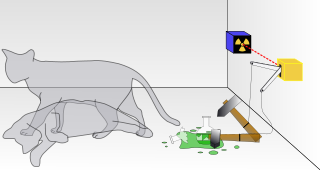
\includegraphics[scale = 0.5]{schrodingers_cat}
		\caption{薛定谔的猫}
		\label{fig.cat}
\end{figure}
把一只猫,一个装有氰化氢气体的玻璃烧瓶和一个放射性原子核放进封闭的盒子里, 如图\ref{fig.cat}所示.当盒子内的监控器侦测到衰变粒子时,就会打破烧瓶,杀死这只猫.
根据量子力学的哥本哈根诠释,在实验进行一段时间后,猫会处于又活又死的叠加态.
可是,假若实验者观察盒子内部,他会观察到一只活猫或一只死猫,而不是同时处于活状态与死状态的猫.
这事实引起一个谜题:到底量子叠加是在什么时候终止,并且坍缩成两种可能状态中的一种状态?

常规计算机存储器有一个问题, 就是他们存储的数据会偶尔翻转, 例如, 宇宙射线就是因其这种错误的一个原因. 为了解决这个问题, 计算机工业研制了一整套错误检测和更正的技术. 一个简单的例子是"校验"检查. 对于量子计算机而言, 也存在这样的问题.

量子输运quantum teleportation, 又叫量子远程传物

量子计算机和量子输运非常依赖\textbf{EPR纠缠态}.

量子信息学告诉人们:为了进行远距离的量子密码通信或量子态隐形传输,人们需要事先让距离遥远的两地共同拥有最大的"量子纠缠态".
所谓"量子纠缠"是指不论两个粒子间距离多远,一个粒子的变化都会影响另一个粒子的现象,即两个粒子之间不论相距多远,从根本上讲它们还是相互联系的.
例如,一个无自旋的粒子分裂成两个粒子,它们的自旋一定相反.但在观测到它们的自旋前,它们是随机的,对一个粒子的观测会瞬时影响到另一个粒子.
科学家们认为,这是一种"神奇的力量", 超距作用,爱因斯坦都无法解释,将其戏称为"遥远的鬼魅行为".
它可成为具有超级计算能力的量子计算机和"万无一失"的量子保密系统的基础.\\
两个伽马光子对撞,有一定的几率产生一对正反电子对,这两个正负电子就处于纠缠态.
\chapter{Quantique}
\section{Equation de Schr\"ondinger}
推广到三维情况下,方程为:
$$
\psi \left({\mathbf r}, t \right) = A \cos \left({\mathbf k} \cdot {\mathbf r} - \omega t + \varphi \right)
$$
其中:
r是三维空间中的位置矢量,
$\cdot$ 是矢量点积,
k是波矢.
这一方程描述了平面波.一维情况下,波矢的大小是角波数
$$|{\mathbf k}| = 2\pi/\lambda$$
波矢的方向是平面波行进的方向.

波动方程是双曲形偏微分方程的最典型代表,其最简形式可表示为:关于位置$x$ 和时间$t$ 的标量函数$u$(代表各点偏离平衡位置的距离)满足:
$$
\dfrac{\partial^2 u}{\partial t^2} = c^2 \nabla^2u
$$
这里c通常是一个固定常数,代表波的传播速率.
在针对实际问题的波动方程中,一般都将波速表示成可随波的频率变化的量,这种处理对应真实物理世界中的色散现象.此时,$ c$  应该用波的相速度代替:$v_\mathrm{p} = \frac{\omega}{k}$

上面的波动方程可以化成下面的形式
$$
\left(\nabla^2-\frac{1}{c^2}\frac{\partial^2}{\partial{t}^2}\right)u(\mathbf{r},t)=0.
$$
Separation of variables begins by assuming that the wave function $u(r, t)$ is in fact separable:
$$u(\mathbf{r},t)=A (\mathbf{r}) T(t)$$
Substituting this form into the wave equation, and then simplifying, we obtain the following equation:
$$\dfrac{\nabla^2 A}{A} = \dfrac{1}{c^2 T } \dfrac{d^2 T}{d t^2}$$
Notice the expression on the left-hand side depends only on $r$ , whereas the right-hand expression depends only on $t$.
As a result, this equation is valid in the general case if and only if both sides of the equation are equal to a constant value. 
From this observation, we obtain two equations, one for $A(r)$ , the other for $T(t)$ :
$$\dfrac{\nabla^2 A}{A} = -k^2$$
and
$$\dfrac{1}{c^2 T } \dfrac{d^2 T}{d t^2} = -k^2$$
Rearranging the first equation, we obtain the Helmholtz equation:
$$\nabla^2 A + k^2 A  =  ( \nabla^2 + k^2)  A  =  0$$
Likewise, after making the substitution
$$ \omega  \stackrel{\mathrm{def}}{=}  kc $$
the second equation becomes
$$\frac{d^2{T}}{d{t}^2} + \omega^2T  =  \left( \dfrac{d^2 }{dt^2 } + \omega^2 \right) T  =  0,$$
where $k$ is the wave vector and $\omega$ is the angular frequency.\par
我们可以解出
$$
T(t) = \exp^{-i \omega t}
$$

回到第一个方程\par
La longueur d'onde dans le milieu est d\'efinie par $\lambda = 2 \pi/k$. L'\'equation de Helmholtz se r\'e\'ecrit :

$$
\left( \, \Delta \ + \ \frac{4\pi^2}{\lambda^2} \, \right) \ \psi(\vec{r}) \ = \ 0
$$

On utilise alors la relation de de Broglie pour une particule non relativiste, pour laquelle la quantit\'e de mouvement $p = m v$  :
$$
\lambda \ = \ \frac{h}{mv} \quad \Longrightarrow \quad \frac{1}{\lambda^2} \ = \ \frac{m^2 \, v^2}{h^2}
$$

Or, l'\'energie cin\'etique s'\'ecrit pour une particule non relativiste :
$$
\frac{1}{2} \, m \, v^2 \ = \ E \ - \ V(\vec{r})
$$

d'où l'\'equation de Schr?dinger stationnaire :
$$
\left[ \, \Delta \ + \ \frac{8\pi^2m}{h^2} \, \left( \, E \ - \ V(\vec{r}) \, \right) \ \right] \ \psi(\vec{r}) \ = \ 0
$$

En introduisant le quantum d'action $\hbar = h/2\pi$, on la met sous la forme habituelle :
$$
- \ \frac{\hbar^2}{2m} \, \Delta \psi(\vec{r}) \ + \ V(\vec{r}) \, \psi(\vec{r}) \ = \ E \, \psi(\vec{r})
$$

Il ne reste plus qu'\`a r\'eintroduire le temps t en explicitant la d\'ependance temporelle pour une onde monochromatique, puis en utilisant la relation de Planck-Einstein $E = \hbar \omega$:

$$
\psi(\vec{r},t) \ = \ \psi(\vec{r}) \ \mathrm{e}^{- \, i \, \omega \, t} \ = \ \psi(\vec{r}) \ \exp \left( - \, \frac{i \, E \, t}{\hbar} \right)
$$

On obtient finalement l'\'equation de Schr\"odinger g\'en\'erale :
$$
- \ \frac{\hbar^2}{2m} \, \Delta \psi(\vec{r},t) \ + \ V(\vec{r}) \, \psi(\vec{r},t) \ = \ i \, \hbar \ \frac{\partial \psi(\vec{r},t)}{\partial t}
$$


L'\'electron est trait\'e comme une onde $\Psi(r,t)$ se d\'epla\c cant dans un puits de potentiel $V$.
La densit\'e de probabilit\'e $\rho(r,t)$ qui lui est associ\'ee est d\'efinie par
$$
\rho(r,t)= R(r,t)^2 = |\Psi(r,t)|^2=\Psi^*(\mathbf{r},t)\Psi(\mathbf{r},t)\,\!
$$
(probabilit\'e par unit\'e de volume, * indique un complexe conjugu\'e)

\section{Le moment cine\'etique: l'orbital et l'intrins\`eque}
\noindent
$L_+ = L_x + i L_y$\\
$L_{\_} = L_x - i L_y$\\
$L^2\ket{\lambda^2,\mu} = \lambda^2 \hbar^2 \ket{\lambda^2,\mu}$\\
$L_z\ket{\lambda^2,\mu} = \mu \hbar \ket{\lambda^2,\mu}$

求$\norm{L_+\ket{\lambda^2, \mu}}$
$$
\norm{L_+ \ket{\lambda^2,\mu}}^2 = \braket{\lambda^2,\mu}{L_+^+ L_+}{\lambda^2,\mu}
$$
$$
L_+^+ = L_x - i L_y = L_{\_}
$$
\begin{equation}
\begin{aligned}
L_{\_} L_+ 
& = (L_x - i L_y)(L_x + i L_y)\\
& = L_x^2 + L_y^2 + i(L_x L_y - L_y L_x)\\
& = L_x^2 + L_y^2 + i[L_x, L_y]\\
& = L_x^2 + L_y^2 - \hbar L_z
\end{aligned}
\end{equation}

\begin{equation}
\begin{aligned}
\norm{L_+ \ket{\lambda^2,\mu}}^2 
& = \braket{\lambda^2,\mu}{L_+^+ L_+}{\lambda^2,\mu}\\
& = \braket{\lambda^2,\mu}{L_x^2 + L_y^2 - \hbar L_z}{\lambda^2,\mu}\\
& = \braket{\lambda^2,\mu}{L^2 - L_z^2 - \hbar L_z}{\lambda^2,\mu}\\
& = \braket{\lambda^2,\mu}{L^2}{\lambda^2,\mu}
- \braket{\lambda^2,\mu}{L_z^2}{\lambda^2,\mu}
- \braket{\lambda^2,\mu}{\hbar L_z}{\lambda^2,\mu}\\
& = \hbar^2(\lambda^2 - \mu^2 - \mu)
\end{aligned}
\end{equation}
Donc, $\norm{L_+ \ket{\lambda^2,\mu}} = \hbar \sqrt{\lambda^2 - \mu^2 - \mu}$\\
Donc, $\norm{L_{\_} \ket{\lambda^2,\mu}} = \hbar \sqrt{\lambda^2 - \mu^2 + \mu}$\\
从模非负可以推出$\mu^2 < \lambda^2$

求$L_+\ket{\lambda^2, \mu}$ 的方向
\todo{这里不知道为什么不显示}
$$
\begin{aligned}
[L_z, L_+]
& = [L_z, L_x + i L_y] \\
& = [L_z, L_x] + i [L_z, L_y] \\
& = i\hbar L_y + i(-i\hbar L_x) \\
& = \hbar (L_x + i L_y) \\
& = \hbar L_+
\end{aligned}
$$

\begin{equation}
\begin{aligned}
L_zL_+\ket{\lambda^2,\mu}
& = (L_+L_z + \hbar L_+)\ket{\lambda^2, \mu} \\
& = L_+L_z\ket{\lambda^2, \mu} + \hbar L_+\ket{\lambda^2, \mu} \\
& = L_+ \hbar \mu \ket{\lambda^2, \mu} + \hbar L_+\ket{\lambda^2, \mu} \\
& = \hbar (\mu + 1) L_+ \ket{\lambda^2, \mu}
\end{aligned}
\end{equation}
考虑到$L_z \ket{\lambda^2,\mu + 1} = \hbar (\mu+1)\ket{\lambda^2,\mu+1}$, 和\lasteq 对比, 可以推出
$$
L_+\ket{\lambda^2,\mu} \varpropto \ket{\lambda^2,\mu+1}
$$
结合前面求出的模, 我们得出
$$ L_+ \ket{\lambda^2,\mu} = \hbar \sqrt{\lambda^2 - \mu^2 - \mu}\ket{\lambda^2, \mu+1} $$
$$ L_{\_} \ket{\lambda^2,\mu} = \hbar \sqrt{\lambda^2 - \mu^2 + \mu}\ket{\lambda^2, \mu-1} $$
